%%%%%%%%%-----------------------------------------------------------------
%%%%%%%%% Thesis template, v1
%%%%%%%%% Mathematical & Statistical Methods group - Biometris
%%%%%%%%% Wageningen University & Research
%%%%%%%%%-----------------------------------------------------------------


\documentclass{amsart}

\usepackage{booktabs}
\usepackage{lipsum}
\usepackage{multicol}

% Setting margins
\usepackage[a4paper, left=3cm,right=3cm]{geometry}

% Packages for the titlepage
\usepackage{tikz}
\usetikzlibrary{calc}
\usepackage{graphicx}
\usepackage{newtxtext}
\usepackage{float}
\usepackage{svg}

% Packages for mathematical writing
\usepackage{amsmath}                           % Enables the align enviroment
\usepackage{amssymb}                           % Math symbols (e.g. \mathbb{})
\usepackage{dsfont} 	                         % For \mathds{1} blackboard bold 1
\usepackage{bm}                                % For roman (upright) bold latin letters
\usepackage{mathtools}                         % Better math
\usepackage[hypertexnames=false]{hyperref}     % For urls and hyperlinks
\usepackage[scientific-notation=true]{siunitx} % For scientific notation
\usepackage{euscript}[mathcal]
\usepackage{txfonts}

% For theorems, remarks, lemmas etc.
\usepackage{amsthm}
\theoremstyle{plain}
\newtheorem{theorem}{Theorem}%[section]
%% >> Define your newtheorems here

% For algorithms
\usepackage[ruled,vlined]{algorithm2e}
\usepackage{algpseudocode}
\renewcommand{\algorithmicrequire}{\textbf{Input:}}
\renewcommand{\algorithmicensure}{\textbf{Output:}}

% Often used math operators:
% You can define these yourself using \DeclareMathOperator and \newcommand
%\DeclareMathOperator*{\argmax}{arg\,max}    % maxmizing argument
%\newcommand{\LA}{\mathbf{\Lambda}}

% For bibliography
\usepackage[
    backend=biber,
    style=nature, 
    maxcitenames=1,
    mincitenames=1]
    {biblatex}
\addbibresource{references.bib}
\addbibresource{entries.bib}
\def\bibfont{\footnotesize}
\usepackage[acronym, nomain]{glossaries}
\makeglossaries

\newacronym{ad}{AD}{Alzheimer's Disease}
\newacronym{scd}{SCD}{Subjective Cognitive Decline}
\newacronym{mci}{MCI}{Mild Cognitive Impairment}
\newacronym{sad}{SAD}{sporadic Alzheimer's Disease}
\newacronym{fad}{FAD}{familial Alzheimer's Disease}
\newacronym{apoe}{ApoE}{Apo-lipoprotein E}
\newacronym{load}{LOAD}{late-onset Alzheimer's Disease}
\newacronym{idl}{IDL}{intermediate density lipoprotein}
\newacronym{vldl}{VLDL}{very low density lipoprotein}
\newacronym{abca1}{ABCA1}{ATP-binding cassette transporter A1}
\newacronym{lrp}{LRP1}{low density lipoprotein receptor-related protein 1}
\newacronym{hdl}{HDL}{high density lipoprotein}
\newacronym{bbb}{BBB}{blood-brain barrier}
\newacronym{tlr4}{TLR4}{toll-like receptor 4}
\newacronym{nfkb}{NFkB}{nuclear factor kappa B}
\newacronym{atp}{ATP}{Adenosine tri-phosphate}
\newacronym{vcs}{VCS}{Version Control System}
\newacronym{cv}{CV}{Cross-Validation}
\newacronym{gsk}{GSK-3$\beta$}{Glycogen synthase kinase-3$\beta$}
\newacronym{csf}{CSF}{cerebrospinal fluid}
\renewcommand*{\glossarymark}[1]{}
\setcounter{tocdepth}{3}


%--------------------------------------------------------------------
%--------------- Front and Main matter style ------------------------
\newcommand{\frontmatter}{
    \pagenumbering{roman}   % Setting page numbering to lower-case roman
}
\newcommand{\mainmatter}{
    \newpage
    \pagenumbering{arabic}  % Setting page numbering to normal integers
}
%--------------- Front and Main matter style ------------------------
%--------------------------------------------------------------------

\begin{document}
% \Sconcordance{concordance:Thesis_Template_Biometris.tex:Thesis_Template_Biometris.rnw:1 %
65 1 1 0 345 1 1 9 11 0 1 2 136 1}



% Add title page:
%------------------------------------------------------------------------------
% In this segment, enter the desired student data to be shown at the title page
\newcommand{\thesisAuthor}{George Miliarakis}                             % State your name
\newcommand{\thesisTitle}{Mechanistic insights into ApoE4 dose effects on serum metabolites in Alzheimer's Disease}                                      % State title thesis
\newcommand{\thesisSubTitle}{a Data Science approach}                            % State subtitle thesis
\newcommand{\thesisDegree}{MSc Thesis}      % Choose type
\newcommand{\university}{Wageningen University \& Research}                % You generally don't need to touch this
\newcommand{\thesisPlaceDate}{Wageningen, December 2023}                      % State month and year
%------------------------------------------------------------------------------


%------------------------------------------------------------------------------
% In this segment, enter the desired supervisor data to be shown at the title page
\newcommand{\supervisor}{C.F.W. Peeters}                                                % State name of supervisor
\newcommand{\departmentSUP}{Mathematical \& Statistical Methods (Biometris)} % State department supervisor (generally Biometris)
\newcommand{\universitySUP}{Wageningen University \& Research}                              % State university supervisor (generally WUR)
%------------------------------------------------------------------------------


%------------------------------------------------------------------------------
% In this segment, enter the desired co-supervisor data to be shown at the title page
\newcommand{\cosupervisor}{Yannick Vermeiren}                                         % State name of co-supervisor
\newcommand{\departmentCOSUP}{Nutrition, Brain and Cognitive Ageing}                             % State department or division co-supervisor
\newcommand{\universityCOSUP}{Wageningen University \& Research}                              % State university or company co-supervisor
%------------------------------------------------------------------------------


%------------------------------------------------------------------------------
% Logos and visuals
\begin{titlepage}
\thispagestyle{empty}

% Adding logos
\begin{figure} [H]
\vspace{-3cm}
 \centering
\begin{minipage}[t]{.45\linewidth}
  \raggedright
  % Upload and include SLU loggo here:
  \hspace*{-2cm}
\includegraphics[width=\linewidth]{figures/WURlogo.png}

\end{minipage}%
  \begin{minipage}[t]{.45\linewidth}
  \vspace{-2.6cm}
 \raggedleft
%% Inclusion Biometris logo
 \hspace*{+2cm}
\includegraphics[width =.95\textwidth]{figures/biometris_logo.png}

\end{minipage}
\end{figure}

% Bottom/background picture
\begin{tikzpicture}[overlay, remember picture]
\node[anchor=south west,
      xshift=+6.5cm,
      yshift=-0.2cm]
     at (current page.south west)
     {
\includegraphics[width = 0.5\textwidth]{figures/torontodeclaration.png}};
\end{tikzpicture}
%------------------------------------------------------------------------------


%------------------------------------------------------------------------------
% Title information
\vspace{1cm}
\begin{center}
\par
\noindent
\rule[0.2cm]{\linewidth}{1.5pt}
\Huge
\textbf{\thesisTitle}
\vspace{0.2cm}
\LARGE
\par
\noindent
\thesisSubTitle\\
\rule[0.2cm]{\linewidth}{1.5pt}
\Large
\end{center}
%------------------------------------------------------------------------------


%------------------------------------------------------------------------------
% Author information
\vspace{2cm}
\noindent
\LARGE
\thesisAuthor\\
\vspace{.2 cm}
\small
\par \noindent
\thesisDegree
\par \noindent
\university
\par \noindent
\thesisPlaceDate
%------------------------------------------------------------------------------


%------------------------------------------------------------------------------
% Supervision information
\vspace{4cm}
\begin{flushright}
\emph{Supervisor} \\
\textbf{\supervisor} \\
\departmentSUP \\
\universitySUP
\end{flushright}

\vspace{.5cm}
\begin{flushright}
\emph{Supervisor} \\
\textbf{\cosupervisor} \\
\departmentCOSUP \\
\universityCOSUP
\end{flushright}
\end{titlepage}
%------------------------------------------------------------------------------
%--------------- Front matter ---------------------------------------
%-------------------------------------------------------------------
\frontmatter
% Foreword
\section*{Foreword}
This is where you type your foreword.
In the Foreword the student states clearly his/her contribution that originates from the master thesis project, and, if applicable, what contribution(s) possibly followed from the student’s internship on the same topic.
It is also stated in the foreword what data sources were used, and whether the data have a degree of confidentiality.
In addition, possible acknowledgements may be made to people who have contributed to (certain parts of) the thesis.


% Abstract
\newpage
\section*{Abstract}
This is where you type your abstract.
The abstract must be communicable to a broad audience and contain, next to a summary text, an outreach item such as an infographic or a link to a video/website/web application.
Such as, for example, the nice figure below.


% Glossary
\clearpage
\printacronyms[title = Abbreviations, toctitle = Abbreviations]

\newpage
% Inserting table of contents
\tableofcontents

%--------------------------------------------------------------------
%--------------- Main matter ----------------------------------------
\mainmatter

\newpage
\section{Introduction}\label{Intro}
\subsection{Alzheimer’s Disease}
Alzheimer’s Disease (AD) is a complex, progressive neurodegenerative disorder and the most common form of dementia \cite{Penke2023NewDisease}. It was considered the 6th leading cause of death in the US in 2019, with an overall increase of 145\% in mortality from 2000 to 2019 \cite{20232023Figures}. The impact AD has on patients, their caregivers, and healthcare systems is detrimental. In 2022, caregivers of people with AD or other dementias provided an estimated 18 billion hours of unpaid assistance, valued at \$339.5 billion, more than 14 times the total revenue of McDonald's in 2022 (\$23.3 billion) \cite{20232023Figures}. Its estimated annual global societal cost exceeds the GDP of The Netherlands \cite{Wimo2023The2019}. Despite decades of research, factors to prevent, slow or cure AD remain to be discovered.

The main risk factor for AD is age, while several genetic and lifestyle risk factors, as well as biochemical pathways contribute to its development \cite{Penke2023NewDisease}. AD occurs in various histopathological phenotypes and presents a broad spectrum of clinical signs and symptoms \cite{Heneka2015NeuroinflammationDisease, Edwards2019ANeurodegeneration}. The AD continuum starts with subjective cognitive decline (SCD), followed by mild cognitive impairment (MCI) \cite{Rasmussen2019AlzheimersDiagnosis}, and continues with progressive loss of global cognition, of which particularly memory, processing speed and executive functioning, spanning a total period of 10-15 years \cite{Scheltens2016AlzheimersDisease}. 

The most common phenotype of AD is sporadic or late-onset AD (\acrshort{sad}, \acrshort{load}; \>95\% of cases), typically appearing after 65 years of age \cite{Beydoun2014EpidemiologicMeta-analysis}. A rarer phenotype is early-onset familial AD (\acrshort{fad}), usually starting at ages 30–65 and passed in an autosomal dominant fashion \cite{VanCauwenberghe2015ThePerspectives}.
Even though FAD mutations explain only a small percentage of AD cases, they have a great impact on AD research given their appealing genotype-phenotype links.

\subsubsection{Amyloid cascade hypothesis}
The amyloid cascade hypothesis has been the most predominant in explaining the pathogenesis of AD. In historical terms, its impact was profound, as it helped distinguish and identify AD as a single disease that may be studied for treatment \cite{Hardy2006AlzheimersReappraisal}. It suggests that chronic neuroinflammation promotes protein misfolding and accumulation in the brain, forming plaques (consisting of oligomerized amyloid A$\beta_{42}$) and tangles (consisting of hyperphosphorylated tau protein) \cite{Edwards2019ANeurodegeneration}. Nevertheless, it does not necessarily cover all AD cases; clinical trials of A$\beta$ anti-bodies as treatment prove the amyloid cascade hypothesis as insufficient \cite{Kepp2023TheReview,Kurkinen2023TheThinking}. Evidence suggests that oxidative stress, metabolic abnormalities, atherosclerosis, cardiovascular effects, imbalances of intra-neuronal calcium and other metal ions contribute to the development of AD \cite{Kepp2023TheReview}. \citeauthor{Kepp2023TheReview} propose a more complex and holistic view of AD pathology, by integrating (epi-)genetic, environmental, vascular, neuro-inflammatory and metabolic factors in predictive models \cite{Kepp2023TheReview}.

\subsection{Human apolipoprotein-E gene}
The gene that encodes apolipoprotein-E (ApoE) is the only gene consistently shown associated with LOAD \cite{Corder1993GeneFamilies}. The structure and function of ApoE, as well as how the first defines the latter is described in section \ref{ApoEprot}.

\subsubsection{Tissue expression}
The principal producers of ApoE are hepatocytes in the liver \cite{Mahley2016CentralMetabolism}. In the CNS, ApoE is primarily expressed in glia, astrocytes, cells of which modulate metabolic homeostasis and neuronal communication, followed by microglia, the resident immune cells of the brain \cite{Lanfranco2021ExpressionInflammation}. Each genotype is linked to different expression levels \cite{Husain2021APOETherapeutics}. Carriers of $\varepsilon_2$ seem to have higher \acrfull{CSF} levels of ApoE, compared to $\varepsilon_4$ carriers \cite{Castellano2011HumanClearance, Cruchaga2012CerebrospinalDisease}. 

\subsubsection{ApoE polymorphism is the strongest genetic risk factor for Alzheimer's Disease}
Humans present three variants of the ApoE gene: $\varepsilon_2$, $\varepsilon_3$ and $\varepsilon_4$ \cite{Husain2021APOETherapeutics, Yang2023ApolipoproteinDisease}, resulting in six genotypes [Fig. \ref{fig1}]. In Caucasian populations apo$\varepsilon_3$ (rs7412 C/rs429358 T) is the most abundant, with a frequency of 78\%, and is considered neutral regarding the risk of AD \cite{Liu2013ApolipoproteinTherapy}. Apo$\varepsilon_4$ (rs7412 C/rs429358 C) has a frequency of 14\% and represents the strongest genetic risk factor for LOAD, in a gene dose-dependent manner \cite{Strittmatter1993ApolipoproteinDisease}. Conversely, apo$\varepsilon_2$ (rs7412 T/rs429358 T) is found in 8\% of Caucasian populations, and carriers of this allele exhibit a reduced risk of LOAD \cite{Liu2013ApolipoproteinTherapy}. The various ApoE alleles are strongly linked to the primary pathological features of LOAD, namely amyloid-A$\beta$ and phosphorylated tau \cite{Deming2017Genome-wideModifiers}. While the association between ApoE alleles and LOAD risk or protection is observed across diverse ancestral backgrounds, the strength of this association varies \cite{Belloy2019AForward, Farrer1997EffectsMeta-analysis}, see section 1.2.2.

\begin{figure}[]
  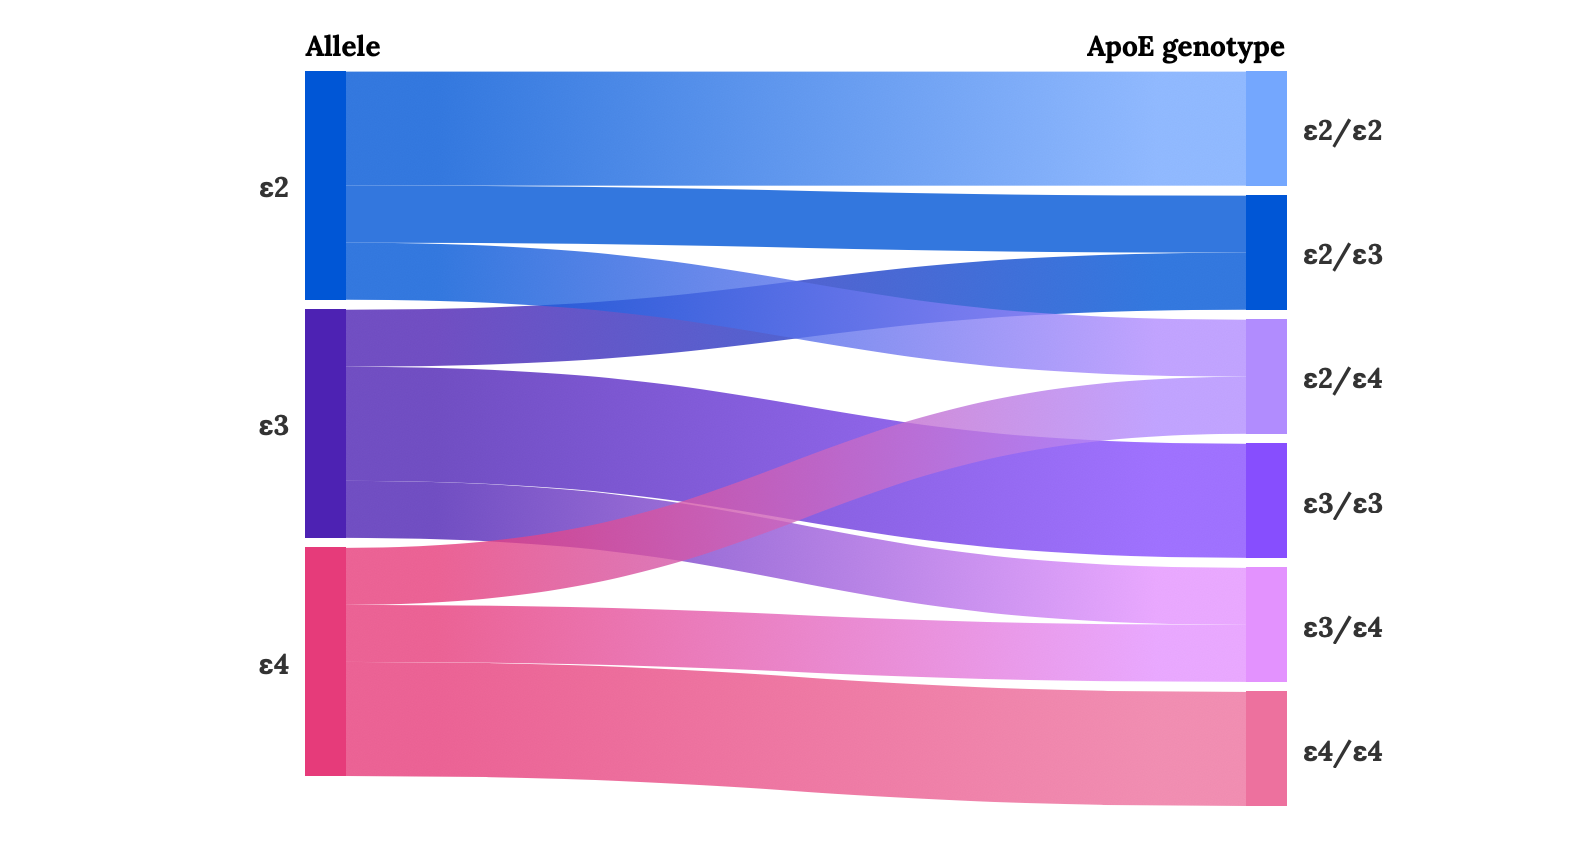
\includegraphics[width=0.7\textwidth]{figures/ApoE@2x.png}
    \caption{Sankey chart showing the allele distribution among the 6 ApoE genotypes.}
  \label{fig1}
\end{figure}

\subsubsection{ApoE and ancestry in Alzheimer's Disease}
The majority of studies exploring the relationship between ApoE alleles and the genetics of LOAD have primarily focused on Northern European populations\cite{Yang2023ApolipoproteinDisease}. However, smaller investigations involving diverse ancestral backgrounds indicate variations in ApoE4 allele frequencies across different populations\cite{Yang2023ApolipoproteinDisease}. While ApoE4 is present in 14\% of Caucasian Americans, its prevalence increases to 40\% among African Americans, 37\% in Oceania, and 26\% in Australia. Southern Asia and Europe exhibit ApoE4 allelic frequencies of less than 10\%, compared with Northern Europe where it rises to 25\% \cite{Belloy2019AForward, Egert2012ApoEFactors, Eisenberg2010WorldwideHistory, Logue2011AAmericans}.

The epidemiological impact of ApoE alleles also differs among populations. In Korea, Japan, and Japanese-American communities, ApoE4 confers a higher risk of LOAD compared to Caucasians \cite{Farrer1997EffectsMeta-analysis}. Conversely, for Native Americans, Hispanic Americans, African Americans, and those of African descent, APOE4 is associated with a lower risk of LOAD than in Caucasian-American populations \cite{Farrer1997EffectsMeta-analysis, Blue2019LocalHispanics, Suchy-Dicey2022APOEStudy, Rajabli2018AncestralPopulations, Naslavsky2022GlobalSample}. A recent study in a Chinese population found that ApoE3 is more protective than ApoE2 \cite{Chen2011ApolipoproteinDisease}. Some of these population-specific effects are attributed to the ApoE haplotype \cite{Blue2019LocalHispanics, Rajabli2018AncestralPopulations}. A recent discovery of a novel locus (19q13.31) could contribute to attenuating ApoE4-mediated AD risk in African Americans \cite{Rajabli2022AAncestry}.

\subsubsection{ApoE and sex synergy in Alzheimer's Disease}
Notably, sex (60\% females) and ApoE4 allelic composition (50\% has at least one $\varepsilon_4$ allele) are the strongest genetic risk factors for SAD \cite{, Arnold2020SexMetabolome}. In this regard, it is shown that the ApoE4 genotype has a larger impact on females, as they present greater impairment of mitochondrial energy production, compared to males \cite{Arnold2020SexMetabolome, Yassine2020APOEDisease}.

\subsubsection{Evolution of ApoE over time}
Interestingly, humans are the only ApoE polymorphic species\cite{Yassine2020APOEDisease}. All other animal species have one ApoE variant, which resembles the human $\varepsilon_3$ allele \cite{Hunsberger2019TheInterventions}. ApoE $\varepsilon_4$ is the oldest human allele, followed by $\varepsilon_3$ and $\varepsilon_2$ \cite{Yassine2020APOEDisease}. In highly infectious environments, with food scarcity and shorter lifespans, $\varepsilon_4$ may be adaptive, reducing mortality \cite{Trumble2017ApolipoproteinBurden}. However, as humans transitioned into modern, less infectious environments, with food abundance and longer life expectancy, $\varepsilon_4$ started to burden the arteries and brain, increasing the risk of diseases related to ageing \cite{Yassine2020APOEDisease}. $\varepsilon_3$ emerged from $\varepsilon_4$ and reflects the shift from a plant-based diet to a meat-based one, where genes adaptive to high meat consumption were and still are vital to regulate increased cholesterol levels \cite{Finch1999TheIsoforms}. 

\newpage
\subsection{Apo-lipoprotein E}\label{ApoEprot}
\subsubsection{Structure and function}
\acrshort{apoe} is a brain-specific lipid-binding glycoprotein of 299 amino-acids (34 kDa) that comprises several types of lipoproteins, i.e., chilomicra, \acrshort{idl} and \acrshort{vldl} \cite{Husain2021APOETherapeutics}. Its main function in the brain is the transport of lipids (mainly cholesterol) through membrane receptors \cite{Yang2023ApolipoproteinDisease}. Moreover, its isoforms have an effect on diverse cellular functions, e.g. synaptic integrity, glucose metabolism, A$\beta$ clearance, \acrfull{bbb} integrity and mitochondrial regulation \cite{Husain2021APOETherapeutics}. How these relate to AD pathology will be elaborated in section \ref{ApoEAD}.



\begin{figure}[]
  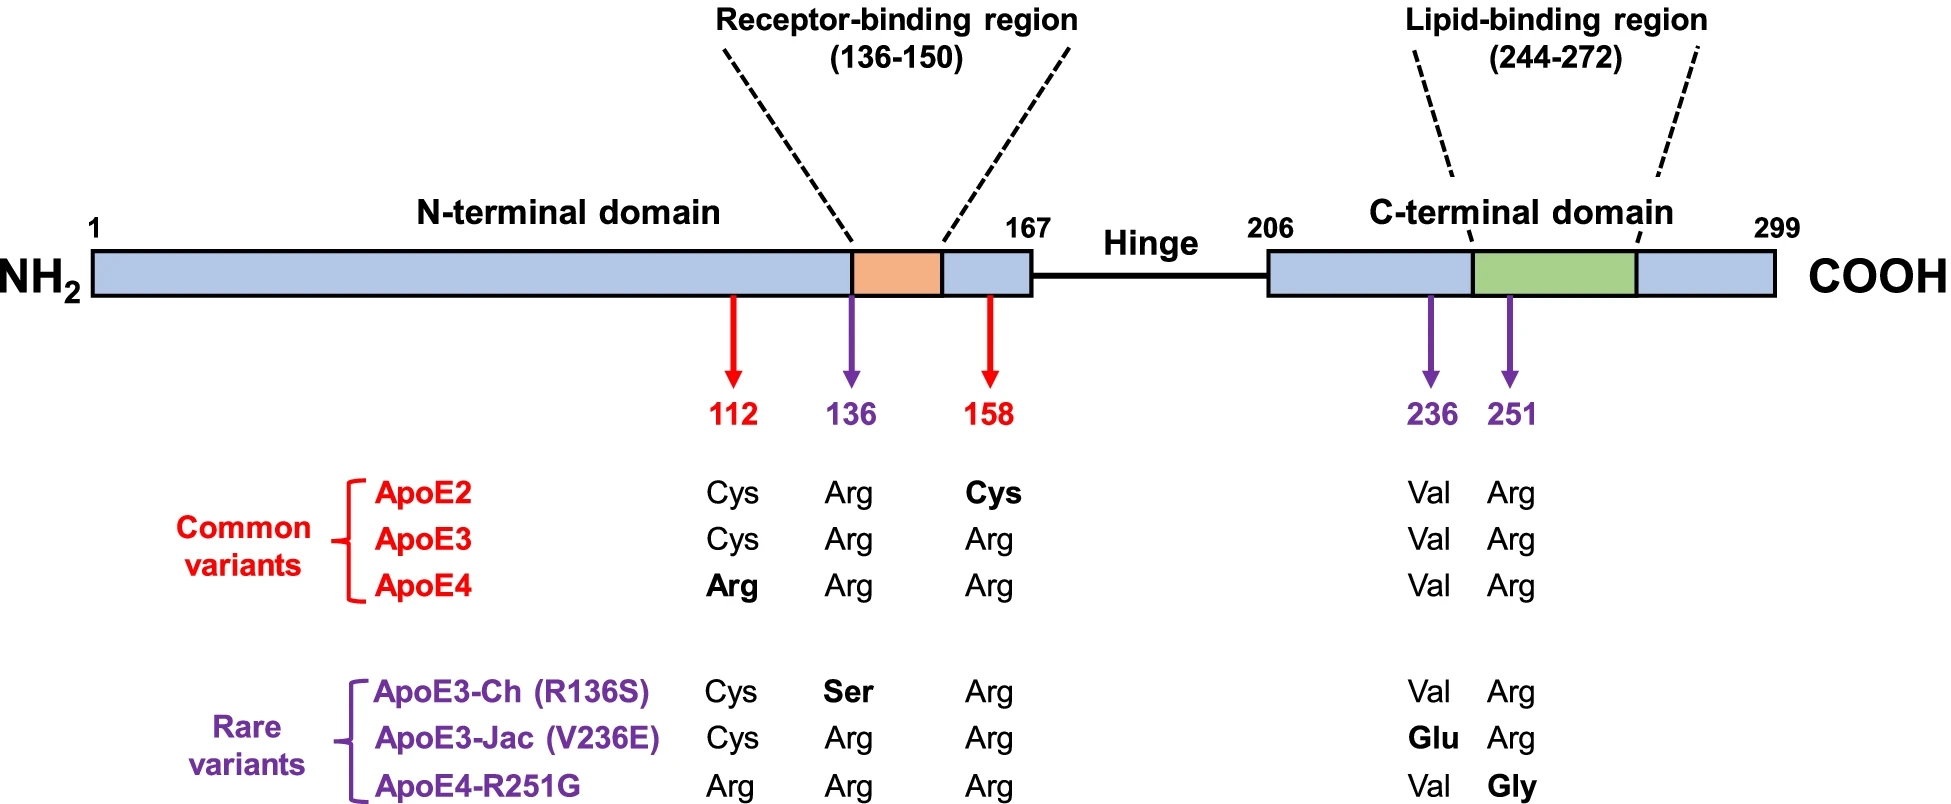
\includegraphics[width=0.8\textwidth]{figures/ApoEprot.png}
    \caption{Linear representation of the ApoE protein. Three structural domains are highlighted: N-terminal, hinge and C-terminal domains. The different aminoacids at positions 112 and 158 are shown per common alleles and aminoacids at positions 136, 236 and 251 coded by rarer alleles. \cite{Bu2022APOEVariants}}
  \label{fig2}
\end{figure}

\subsubsection{ApoE isoforms}
The nuances in the amino acid composition of ApoE, specifically the presence of cysteine or arginine at positions 112 and 158, significantly impact its binding with lipids and receptors \cite{Yassine2020APOEDisease}. The most prevalent isoform, ApoE3, features cysteine at position 112 and arginine at position 158  \cite{Yassine2020APOEDisease}, as shown in Fig. \ref{fig2}. ApoE2 has two cysteines, while ApoE4 has two arginines at these positions \cite{Yassine2020APOEDisease}. The C-terminal domain of ApoE (positions 273–299) is crucial for its lipidation specificity and efficiency \cite{Hu2015OpposingMice}.

\subsubsection{Lipidation nuances of ApoE isoforms}
For ApoE to exert its effects, it needs to be lipidated \cite{Husain2021APOETherapeutics}. ApoE undergoes lipidation via \acrfull{abca1}, a lipid efflux protein \cite{Flowers2020APOEBrain, Courtney2016LXRDisease}. The lipidation degree varies among ApoE isoforms, with ApoE4 exhibiting the least efficient lipidation \cite{Hu2015OpposingMice, Heinsinger2016ApolipoproteinFluid}. This discrepancy in lipidation has been linked to alterations in lipoprotein size and type, in that ApoE4 "prefers" large triglyceride-rich VLDL, while ApoE2 and ApoE3 have a higher affinity for phospholipid-rich \acrshort{hdl} particles \cite{Nguyen2010MolecularE4}. The lower affinity of ApoE4 for HDL particles leads to increased levels of unlipidated ApoE, resulting in its aggregation \cite{Hatters2006ApolipoproteinFunction}. Moreover, ApoE4 fibrils are more neurotoxic than those of ApoE2 and ApoE3 \cite{Hatters2006Amino-terminalFibrils}.

Poor lipidation leads to poor ApoE recycling \cite{Yassine2020APOEDisease}. The latter favors the entrapment of ABCA1 in endosomes, away from the cell membrane, thereby pooling cholesterol in the cell membrane rather than attaching it to HDL particles \cite{Rawat2019ApoE4Astrocytes}. This increased cholesterol content in the cell membrane amplifies \acrfull{tlr4} signaling in macrophages, activating \acrshort{nfkb} and inducing an inflammatory gene response \cite{Yassine2020APOEDisease}.  ApoE4 accumulation also sequestrates insulin receptor (IR) in endosomes, impacting cellular energy preferences \cite{Zhao2017ApolipoproteinEndosomes}. This leads to a decrease in glucose utilization for \acrshort{atp} production and an increase in fatty acid oxidation \cite{Svennerholm1997ChangesSwedes}. 

\begin{figure}[]
  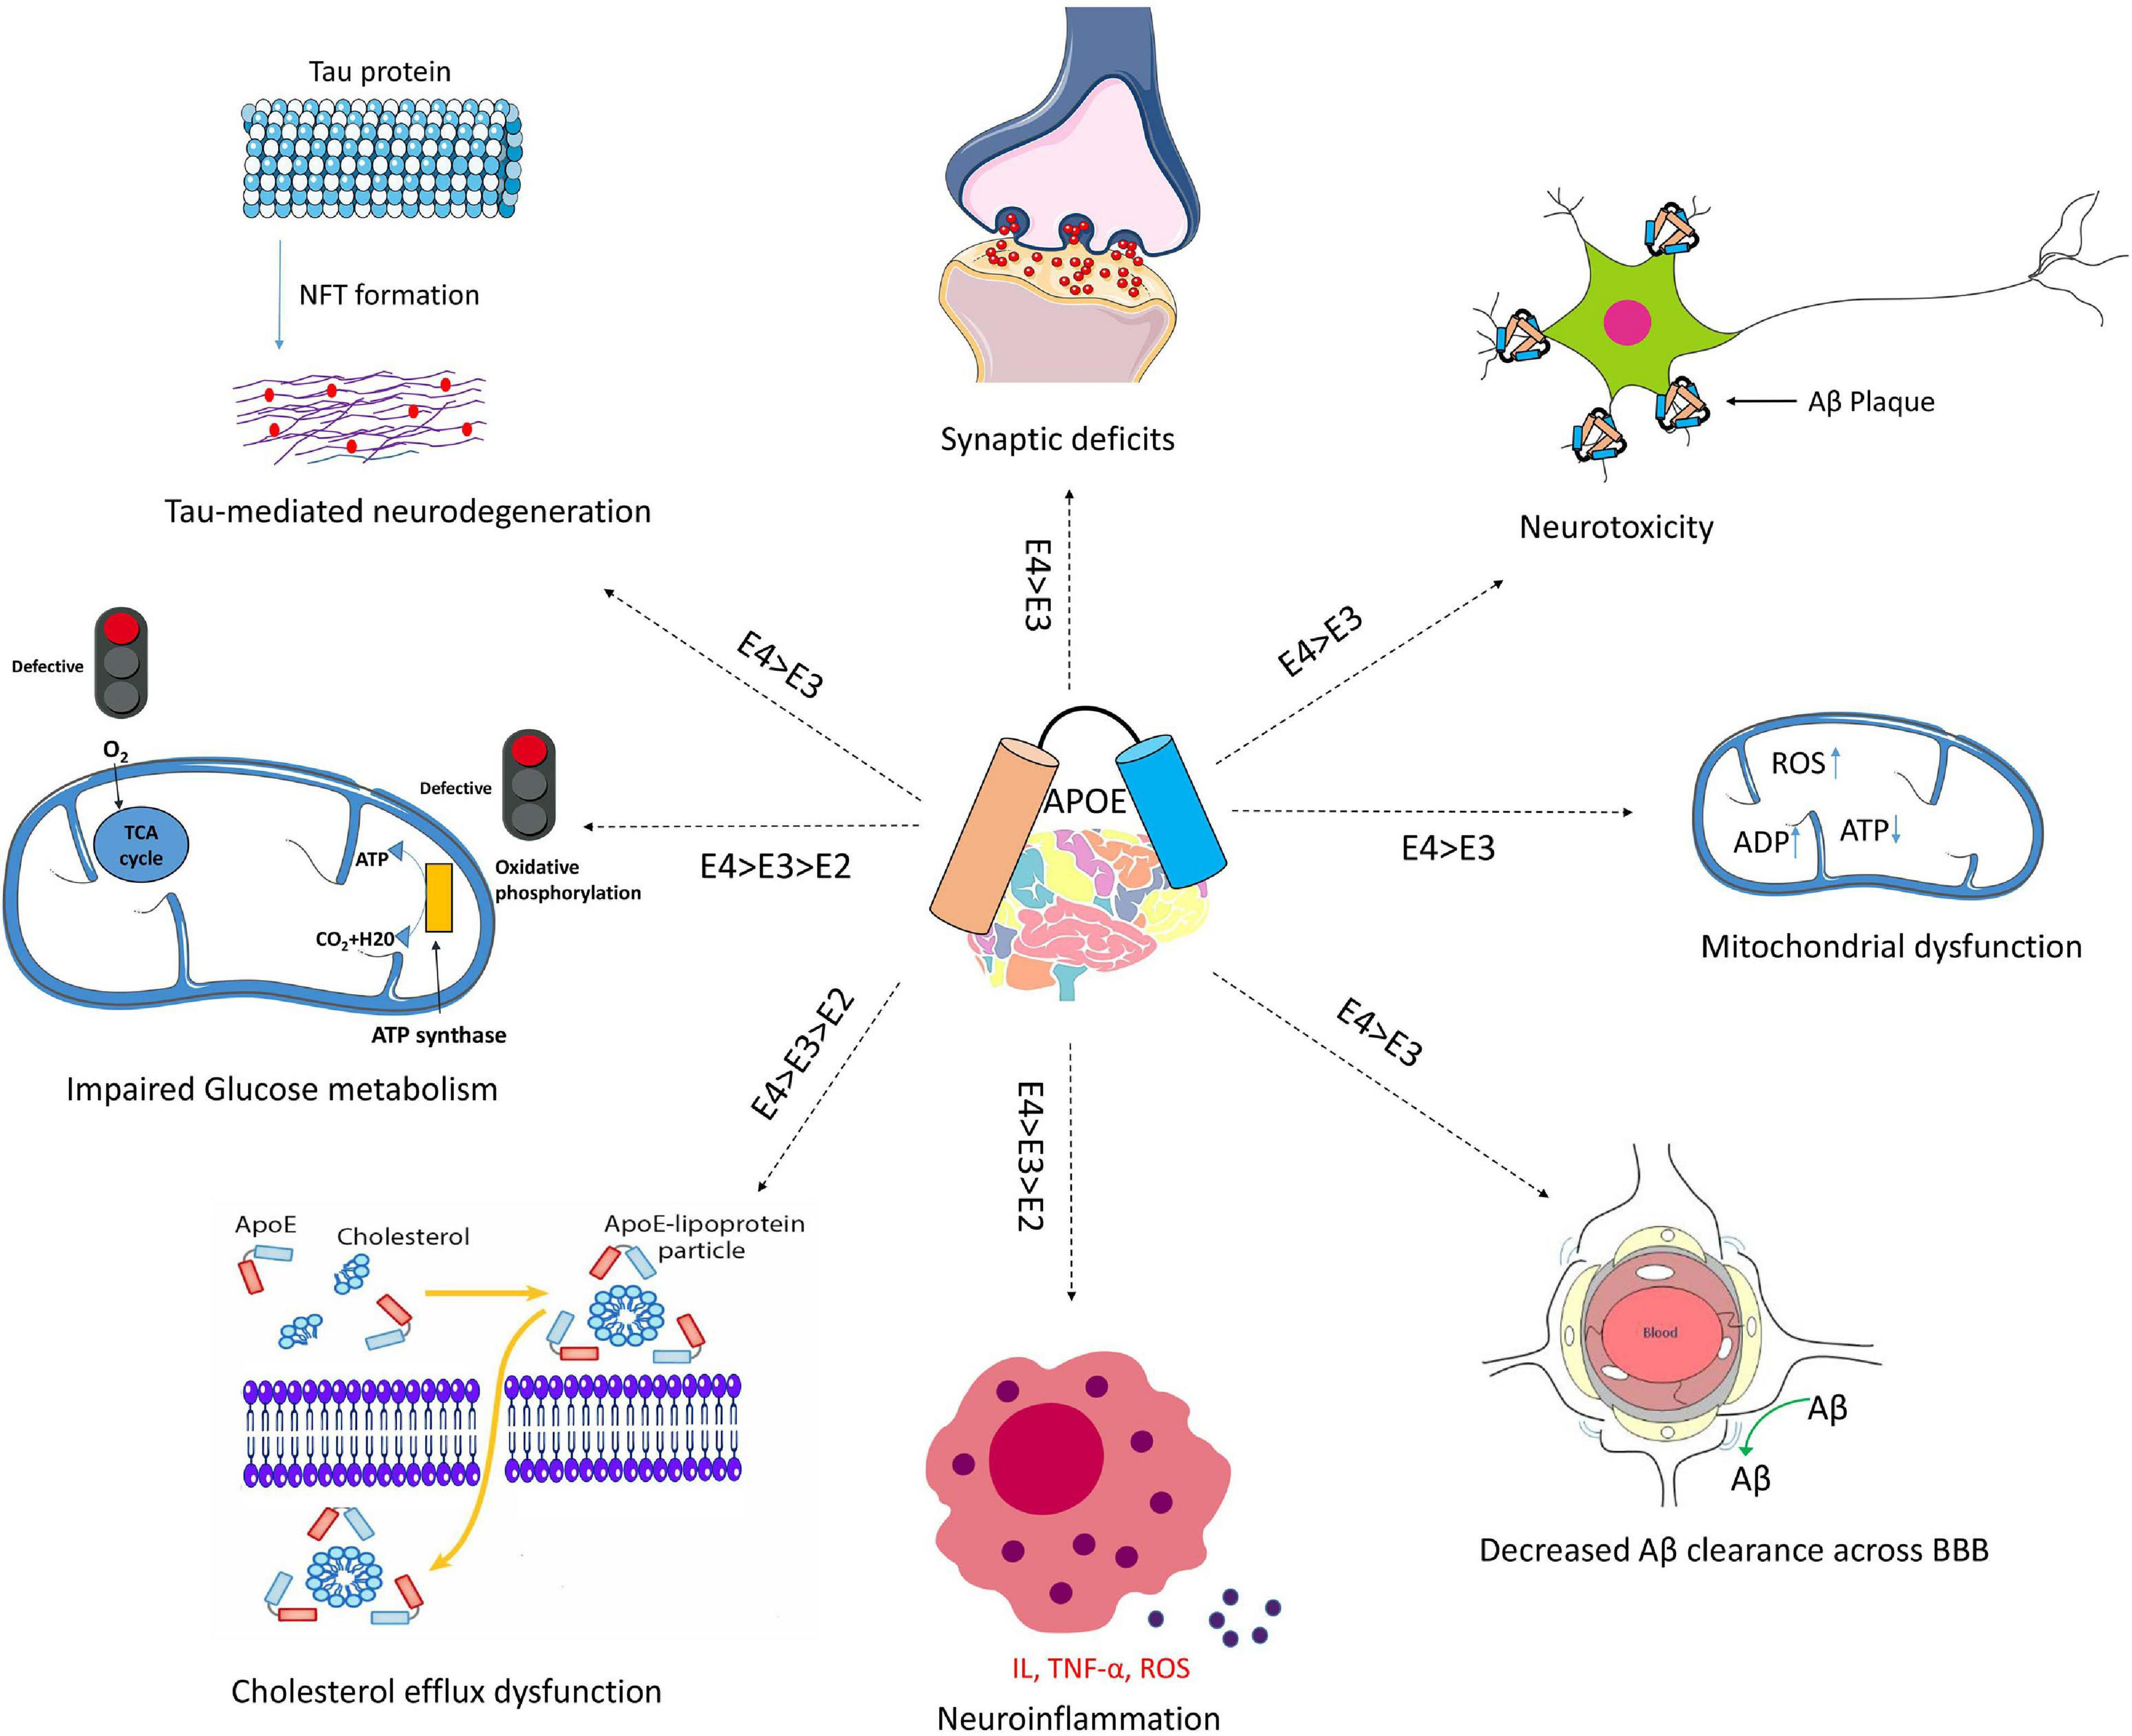
\includegraphics[width=\textwidth]{figures/ApoEeffects.jpg}
    \caption{Schematic overview of A$\beta$-independent effects of ApoE in AD pathology. The isoform-dependent effects of ApoE are indicated. Abbreviations: apoE, apolipoprotein E; NFT, neurofibrillary tangle; BBB, blood brain barrier; IL, interleukin; TNF-$\alpha$, Tumor necrosis factor-$\alpha$; ROS, reactive oxygen species. \cite{Husain2021APOETherapeutics}}
  \label{ApoeEffects}
\end{figure}

\subsubsection{Interplay between ApoE lipidation and Alzheimer's Disease}\label{ApoEAD}
As mentioned earlier, ApoE isoforms have differential pleotropic effects on various cellular functions. ApoE4 induces pro-inflammatory response, leading to the dysfunction of BBB, which in turn impairs cognitive functions \cite{Marottoli2017PeripheralDysfunction, Teng2017ApoEInjury, Kloske2020TheDisease}. Moreover, ApoE modulates the primary neuropathological hallmarks of AD: neuroinflammation, A$\beta$ plaques and tau tangles \cite{Husain2021APOETherapeutics}. Evidence from human and transgenic mice studies reveals increased brain A$\beta$ and amyloid plaque loads in ApoE4 carriers, compared to ApoE3; with the lowest levels in ApoE2 carriers \cite{Huang2017ApoE2Secretion, Tachibana2016RescuingLRP1, Safieh2019ApoE4:Disease}. Higher plaque loads are associated with ApoE4 due to its higher affinity for A$\beta$ and poor clearance capacity \cite{Kloske2020TheDisease}. Additionally, high levels of ApoE4 in neurons remarkably increase tau protein phosphorylation, while high concentrations of ApoE3 don't seem to have an effect \cite{Cao2017ApoE4-associatedInjury, Shi2017ApoE4Tauopathy, Vasilevskaya2020InteractionAthletes, Wang2018GainCorrector}. Notably,  ApoE directly inhibits phosphorylation of tau by \acrshort{gsk} \cite{Hoe2006ApolipoproteinNeurons}. An overview of the A$\beta$-independent effects of ApoE is shown in Fig. \ref{ApoeEffects}.

\subsection{ApoE4-mediated metabolic changes in Alzheimer's Disease}
Metabolism entails the repertoire of chemical reactions that keep living organisms alive. Metabolites  --especially lipid \cite{Barupal2019SetsPathophysiology,Fernandez-Calle2022APOEDiseases, Proitsi2017AssociationAnalysis}-- , perceived as functional intermediates of AD development, are rigorously studied for bio-markers or targets for treatment \cite{Oeckl2019GlialImpairment}.
 
\subsubsection{Measured in \textit{post-mortem} brain tissue}A metabolomic profiling of \textit{post-mortem} brain tissue from AD patients and healthy controls showed  pronounced impairments in sterol and sphingolipid levels in ApoE4 carriers with AD  \cite{Bandaru2009ApoE4Brain}. However, another \textit{post-mortem} metabolomic analysis didn't reveal nuances significantly correlated with ApoE4 \cite{Novotny2023MetabolomicBrains}, although they showed trends in increased cholesterol esters, unsaturated lipids, and sphingomyelin species.

\subsubsection{Measured in blood}
Transcriptomic and lipidomic analyses in humanized ApoE mice associated ApoE4 with decreased free fatty acid levels, many increased  tricarboxylic acid (TCA) cycle metabolites, as well as changes in plasma levels of phosphatidylcholines and unsaturated fatty acids \cite{Area-Gomez2020APOE4Mice, Zhao2020AlzheimersPathways}. A recent study on 58 individuals found six downregulated plasma metabolites (including lysophospholipids and cardiolipin) in ApoE4 carriers \cite{pena-bautista2020MetabolomicsEffect}. Further, the plasma metabolome of the latter reveals a preference for aerobic glycolysis \cite{Farmer2021APO4Glycolysis}. Significant correlations of ApoE genotype and sex with metabolites were observed, i.e. several phosphatidylcholines were found in a large study of more than 1500 individuals \cite{Arnold2020SexMetabolome}

Perturbed serum metabolites associated with AD are amines, aminoacids \cite{deLeeuw2017Blood-basedDisease, Green2023InvestigatingDisease}, cholesteryl esters \cite{Proitsi2017AssociationAnalysis}, sphingolipids \cite{Varma2018BrainStudy,Sun2022AssociationDisease,Green2023InvestigatingDisease,Oeckl2019GlialImpairment,Barupal2019SetsPathophysiology}, fatty acids \cite{Fernandez-Calle2022APOEDiseases,deLeeuw2017Blood-basedDisease}, glycerophospholipids \cite{Varma2018BrainStudy, Jia2022ATypes,Huo2020BrainAnalysis, Weng2019TheImpairment}, phosphatidylcholines \cite{Simpson2016BloodAging} and lipid peroxidation compounds \cite{Fernandez-Calle2022APOEDiseases}. These molecules are usually identified via high-throughput metabolomic pipelines (coupled with Mass Spectrometry (MS) detectors) that trace all compounds in a sample and result in high-dimensional data \cite{Oka2023MultiomicsCohort}. The latter often require advanced statistical methods e.g. projection to latent structures \cite{Weng2019TheImpairment, Peeters2019StableData} or graphical models \cite{Peeters2022Rags2ridges:Matrices} in order to extract putatively meaningful information. 
With such techniques, de Leeuw et al. discovered distinct serum metabolic signatures among AD patients-controls and those carrying at least one ApoE $\varepsilon_4$ allele \cite{deLeeuw2017Blood-basedDisease}, as they appear in Fig. \ref{fig2}. The different metabolic profiles, however, among ApoE4 non-carriers remain obscure. The present data science approach shows ApoE4-mediated differentially expressed metabolites, potentially unveiling distinct pathways of metabolic deregulation in AD.

\begin{figure}
\vspace*{-1cm}
  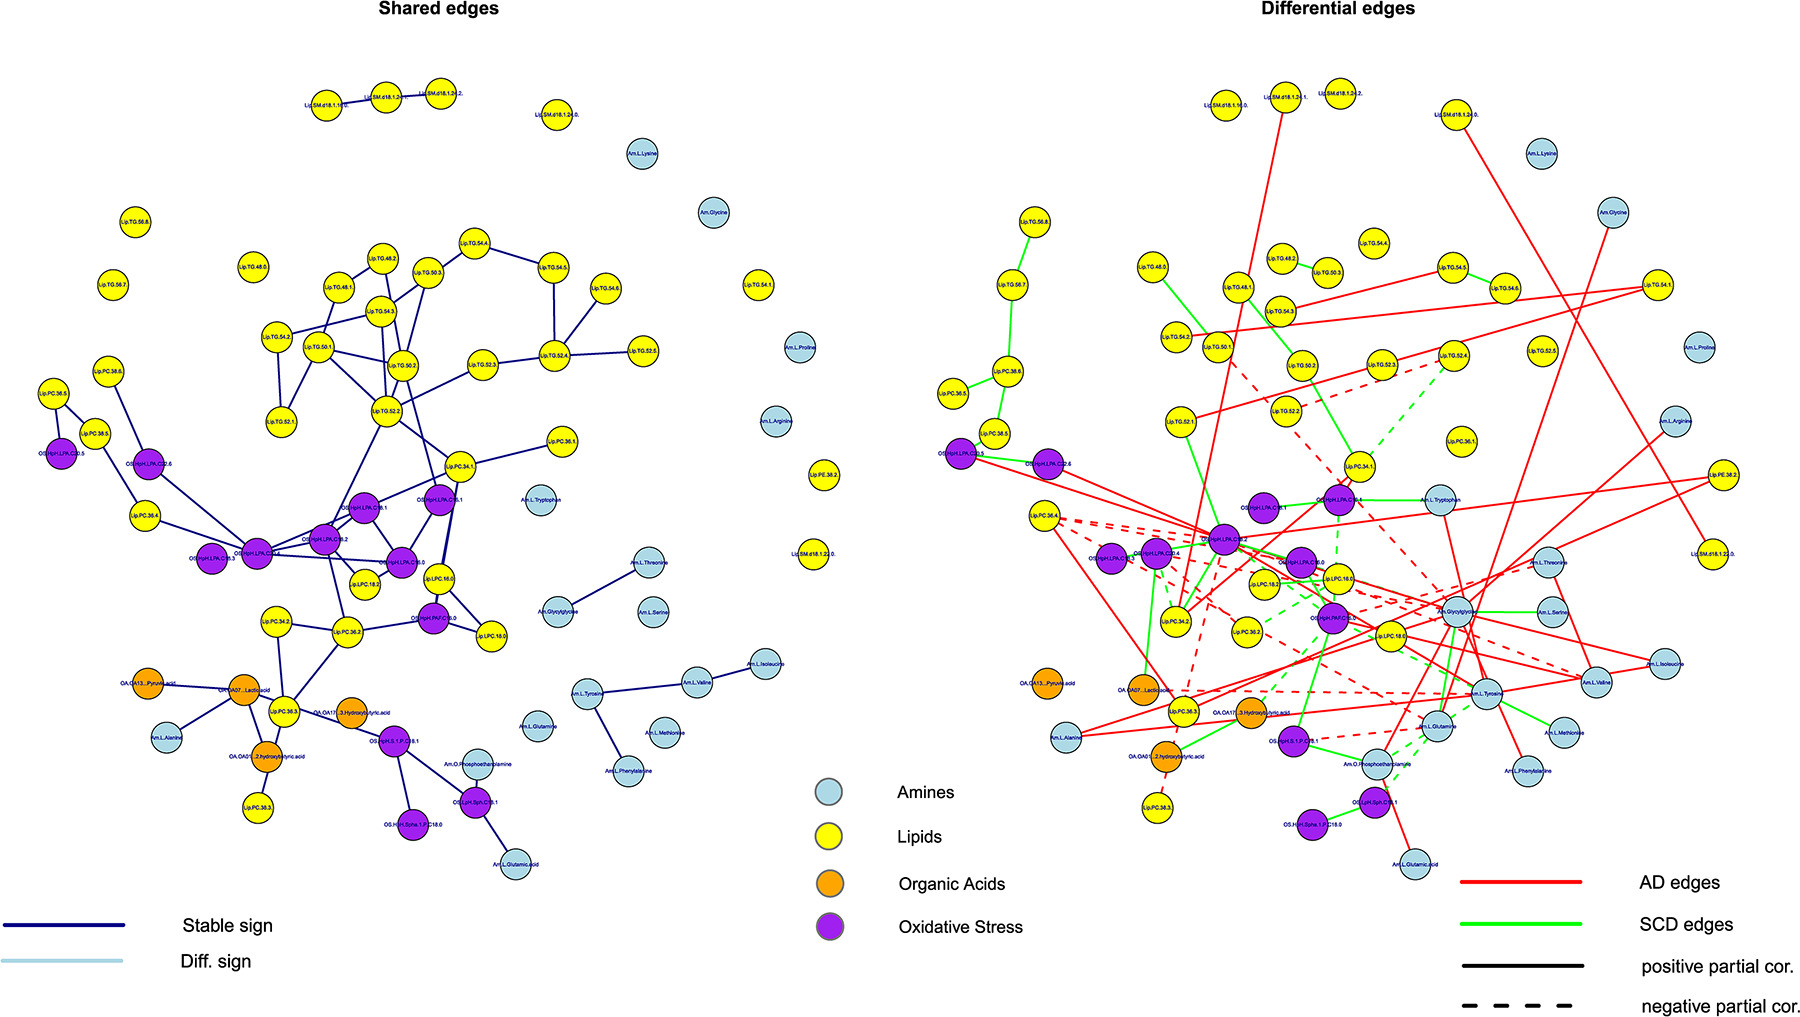
\includegraphics[width=\textwidth]{figures/network.jpeg}
    \caption{Mutual (left-hand panel) and distinct(right-hand panel) metabolic network topologies between ApoE $\varepsilon4$ carriers and non-carriers in AD, as published by de Leeuw et al.. Red edges represent links that are present exclusively in ApoeE $\varepsilon4$ carriers with AD. Green edges represent connections found in the SCD group. Solid edges represent positive partial correlations, while dashed edges represent negative partial correlations. Abbreviations: SCD, subjective cognitive decline }
  \label{fig3}
\end{figure}

\newpage
\subsection{Research Questions}
ApoE $\varepsilon_4$ carriers --particularly females-- experience metabolic disturbances and are at increased risk of SAD. The mechanistic links, however, between ApoE genotype, metabolism and AD development are not entirely known \cite{Fernandez-Calle2022APOEDiseases}, more so among $\varepsilon_4$ non-carriers. Linking specific serum metabolites to distinct ApoE genotypes can reveal metabolic disturbances leading to AD, especially in absence of the ApoE $\varepsilon_4$ allele. Hence, in an effort to elucidate potential links between ApoE genotypes and serum metabolites in AD, one could state the following research questions:

\textbf{RQ}: What are the mechanistic links between ApoE genotype and serum metabolites in AD?
\begin{enumerate}
    \item Are there ApoE4 dose effects in serum metabolite levels?
    \item How discriminatory are serum metabolites among ApoE genotypes?
    \item How do the network topologies of metabolites differ among ApoE genotypes?
\end{enumerate}
\clearpage
\section{Data}
The data were collected from 127 AD patients and 120 SCD ($n$ = 247) individuals in the context of the Amsterdam Dementia Cohort \cite{VanDerFlier2018AmsterdamCare, deLeeuw2017Blood-basedDisease}. In this study two data sets were used: a targeted metabolomics panel and clinical background data, i.e. age at diagnosis, sex, smoking status, alcohol consumption, hypertension (and medication), hyperlipidemia (and medication), anticoagulant medication, anti-depression medication, mean arterial pressure (MAP) and body mass index (BMI). The metabolomics set contains $p =$ 230 metabolites (amines, organic acids, lipids and oxidative stress compounds). The methodology for the metabolomic analysis and ApoE genotyping can be found at de Leeuw et al.'s  Blood-based metabolic signatures in Alzheimer's Disease \cite{deLeeuw2017Blood-basedDisease}: SMT1 . The data was cleaned as described in the same article. The resulting data set is high-dimensional, in the sense that it contains more variables than observations ($p > n$). Another particularity of the data is the covariance and collinearity of the variables. Therefore, appropriate measures need to be taken to prevent model over-fitting --the algorithm being unable to distinguish signal from noise and fitting the latter--  and to correct for spurious correlations.
\newpage
\section{Methodology}
\subsection{Data management}
The FAIR principles for data management and stewardship in science were published by  ~\citeauthor{Wilkinson2016TheStewardship} in 2016 \cite{Wilkinson2016TheStewardship}. FAIR stands for Findable, Accessible, Interactive, and Reusable data; the intention is to create and use data that are well-documented and reproducible. These principles were considered at every step of the study and implemented when applicable. All analysis was performed in R (version 4.3.1), and the current report was written in \LaTeX (Tex Live version 2023). All files are stored in a private Github repository with git as \acrfull{vcs}.

\subsection{Data exploration and Visualisation}
An interactive correlation heatmap was created to visualise the Pearson correlation coefficients using the package \textsf{heatmaply}. 

\subsection{Feature engineering}
The ApoE allele and genotype frequencies in the population are reflected in the AD and SCD data, as shown in Table \ref{Table:ApoEgenfreq}. That is, the most abundant allele is $\varepsilon$3, followed by $\varepsilon4$ and $\varepsilon2$. The most common genotype was $\varepsilon3\varepsilon3$, followed by $\varepsilon3\varepsilon4$ and $\varepsilon4\varepsilon4$.

\begin{table}[h!]
\begin{tabular}{cccccc} \toprule
$\varepsilon2\varepsilon$2 & $\varepsilon2\varepsilon3$ & $\varepsilon2\varepsilon4$ & $\varepsilon3\varepsilon3$ & $\varepsilon3\varepsilon4$ & $\varepsilon4\varepsilon4$ \\ \midrule
2    & 18   & 7    & 106  & 85   & 29   \\ \bottomrule
\end{tabular}
\caption{Individual ApoE genotype counts among SCD and AD patients.} \label{Table:ApoEgenfreq}
\end{table}

The genotypes are not equally represented in the data and hence, don't enable analysis without feature engineering. The following two sections describe the features created to balance the classes when studying only the AD group and both AD and SCD.
\subsubsection{AD group}
An obvious and "low-res" approach would be to bin the samples into two groups: those carrying at least one $\varepsilon4$ allele, and $\varepsilon4$ non-carriers. However, in order to study the $\varepsilon4$ dose effects, the genotypes can be binned into groups, based on the number of $\varepsilon4$ alleles they carry: 0, 1 or 2. The frequencies of $\varepsilon4$ doses are shown in Table \ref{Table:E4binAD}.

\begin{table}[h!]
\begin{tabular}{cccccc} \toprule
$\varepsilon2\varepsilon$2 & $\varepsilon2\varepsilon3$ & $\varepsilon2\varepsilon4$ & $\varepsilon3\varepsilon3$ & $\varepsilon3\varepsilon4$ & $\varepsilon4\varepsilon4$ \\ \midrule
0    & 3    & 2    & 37   & 59   & 26 \\ \bottomrule
\end{tabular}
\caption{Individual ApoE genotype counts among AD patients.} \label{Table:ApoEfreqAD}
\end{table}

\begin{table}[h!]
\begin{tabular}{ccc} \toprule
No $\varepsilon4$  & 1x$\varepsilon4$& 2x$\varepsilon4$\\ \midrule
40    & 61   & 26 \\ \bottomrule
\end{tabular}
\caption{ApoE $\varepsilon4$ dose frequencies among AD patients.} \label{Table:E4binAD}
\end{table}

\subsubsection{SCD and AD}\label{Meth_target}
In order to incorporate the presence of $\varepsilon4$, as well as the diagnosis, a four-level feature ("ApoE4AD") was created, as shown in Table \ref{Table:target}.

\begin{table}[h!]
\begin{tabular}{rcc} \toprule
& $\geq$1 $\varepsilon4$ & no $\varepsilon4$\\ \midrule
AD \vline  & 34& 86\\
 SCD \vline & 87& 40\\ \bottomrule 
\end{tabular}
\caption{Feature combining ApoE4 status and AD diagnosis.} \label{Table:target}
\end{table}
   

\subsection{Statistical Analysis}
The degree to which a user can understand and interpret the prediction or decisions made by a statistical model is defined as \textit{interpretability} \cite{Elshawi2019OnHypertension}. It is of interest in this study to find the optimal balance between the performance of a model with its interpretability. The \textit{bias-variance trade-off} was formally introduced by \citeauthor{Geman1992NeuralDilemma} and refers to the trade-off between the accuracy (opposite of bias) and precision (opposite of variance) of a prediction. It also refers to the trade-off between model flexibility (or complexity) and interpretability \cite{Geman1992NeuralDilemma}.

\subsubsection{ApoE4 dose effects on plasma metabolite levels in AD}
A straight-forward way to test whether metabolites are differentially expressed depending on ApoE4 dose, controlling for clinical variables, is ANOVA (Analysis of Variance) on $p$ nested linear models. The dependent variable in each model is a metabolite; the nested model, eq. \eqref{rm}, has only clinical variables, while the full model, eq. \eqref{fm}, features the clinical variables, plus the number of ApoE4 alleles (0, 1 or 2) as explanatory variables. Let $m_j$ represent the $j$-th metabolite, $x_k$ the $k$-th clinical variable, and D the ApoE4 dose; the nested models then are:
\begin{align}
    & m_j = \beta_0 + \sum_{k=1}^m\beta_kx_k +\varepsilon \label{rm} \\
    & m_j = \beta_0 + \sum_{k=1}^m\beta_kx_k + \beta_{m+1}D_{\varepsilon4} + \varepsilon \label{fm}
\end{align}
Then, for every $j$ = 1,...,$p$ the hypothesis test is H$_0$: $\beta_{m+1} = 0 $ vs H$_\alpha$: $\beta_{m+1} \neq 0$. Under H$_0$ the test statistic, $F$ follows an $F_{1, n-(m+2)}$ distribution. This implies $p$ hypothesis tests, which qualifies as multiple testing. A method to treat the latter is controlling False Discovery Rate \cite{Benjamini1995ControllingTesting}, that is controlling the expected ratio of incorrectly rejected hypotheses, globally e.g. at an $\alpha$ of .05. The caveat of this approach is that minor changes in metabolite levels may not be identified. The next section introduces the concept of a \textit{global test} to deal with this issue.

\subsubsection{Global testing}
A more elegant alternative to multiple testing is global test \cite{Simon2004DesignHealth}. The concept was first introduced by \citeauthor{Simon2004DesignHealth}, and proposed an approach based on permutations to cater to the high dimensionality of gene expression data.

The R package \textsf{GlobalTest} \cite{Goeman2004AOutcome, Goeman2006TestingAlternative, Goeman2023ThePackage} developed by \citeauthor{Goeman2004AOutcome} originally fits a logistic regression model, where the response $Y \in [1,..., k]$ represents two (or $k$) clinical or biological groups and genes are the predictors. This method is also appropriate for other types of -omics data, such as metabolomics in this study \cite{Goeman2023ThePackage}.
The hypothesis test is that metabolite levels are independent of the ApoE4 dose X, i.e. $H_0 : P(Y|X) = P(Y)$, where $X \in \mathbb{R}^{n x p}$. The test statistic of this method employs the low-dimensional (n × n) covariance matrix between samples instead of the large (p × p) covariance matrix between the metabolites. Hence, this method is rather efficient. The test statistic under $H_0$ follows, asymptotically, a normal distribution. In other words, this method tests whether the metabolite levels are discriminating over the dose of ApoE4. The \texttt{gt()} function of the package was used to screen for differences in metabolite levels based on the ApoE4 dose. The \texttt{covariates()} function was used to visualise the ApoE4 dose effects on metabolite levels.

Inspired by global testing, a global ANCOVA method was introduced  by \citeauthor{Mansmann2005TestingApproach} and  extended by \citeauthor{Hummel2008GlobalANCOVA:Effects}, featuring (generalised) linear model comparison based on the extra sum of squares (SS) principle \cite{Hummel2023GlobalExpression}. The null hypothesis tested is that the expression levels are independent of the clinical group membership, i.e. $H_0 : P(X|Y = 1) = P(X|Y = k)$. The high dimensionality is treated by pooling the residual sums of squares (RSS) of gene-level models to the RSS of a global model \cite{Hummel2023GlobalExpression}. The test statistic uses the aggregated RSS and under $H_0$ follows, asymptotically, a $\chi^2$-distribution. The R package \textsf{GlobalAncova} also features a hierarchical generalised linear model comparison function, \texttt{gGlobalAncova.hierarchical()} to fit metabolic pathways. This function was used to test for nuances depending on the 4-class variable ApoE4AD.

\subsubsection{Machine Learning}
The R package \textsf{caret} streamlines the training and comparison of classification and regression models, offering broad parametrization options \cite{Kuhn2008BuildingPackage}. The functions \texttt{trainControl(), train() and confusionMatrix()} were used to fit and evaluate the models. A sampling method used to deal with the unbalanced classes was SMOTE (Synthetic Minority Over-Sampling Technique), as implemented by the package \textsf{DMwR2} \cite{DMwR2}.

Considering interpretability, Multinomial Logistic Regression (MNL) is inherently interpretable. Let $y = k$, with $k \in N, [1,4]$ representing the k-th class of ApoE4AD and $\beta_{kj}$ its set of coefficients,  $\beta_{lj}$ the coefficients of the rest of classes for $j$-th metabolite, then a MNL model calculated the probability

\[\textrm{Pr}(y=k|X=x) =  \dfrac{e^{\sum_{j=1}^{p}\beta_{kj}x_j}}{\sum_{l=1}^{5}\sum_{j=1}^{p}e^{\beta_{lj}x_j}}\]

When $p > n$, the coefficient estimation method has low bias and high variance, in that small changes in the training data can result in very different coefficient estimates \cite{James2023AnEdition}. Regularization trades off a small increase in bias for a great decrease in variance, by shrinking the unimportant coefficients towards zero. LASSO (Least Absolute Shrinkage and Selection Operator) \cite{Tibshiranit1996RegressionLasso}, also called L1-regularization shrinks the MNL coefficients to 0, thus weeding out spurious correlations and reducing the number of predictors \cite{Tibshiranit1996RegressionLasso}. It does so by introducing the term  \[\lambda\sum_{j=1}^{p}|\beta_j|\] where $\lambda \geq 0$ is a tuning parameter that balances the coefficient shrinking effect. The package \textsf{nnet}, as implemented in \textsf{caret}'s \texttt{train()} function was used in this case.

A method to treat multi-collinearity and high dimensionality is a 2-stage Maximum Likelihood(ML) factor analysis (FA), such as the one the package \textsf{FMradio} \cite{Peeters2019StableData} performs. In the 1st stage, a L1-regularised ML estimation is used to filter out redundant features from the data matrix. In the second stage, ML FA projects the aforementioned matrix to an orthogonal space where the features are replaced by -fewer- factors that explain their covariance. One can then use the produced factor scores as predictors in MNL.

Decision Trees (DT) are inherently interpretable, non-parametric models, that fit well large and complicated data sets. They have a tree-like structure that splits the data into branches and leaves(nodes) \cite{Song2015DecisionPrediction}. The \texttt{rpart2()} \cite{rpart} function of \textsf{rpart} was used.

Random Forests (RF) are ensemble learning methods, that bag several DTs and average their decisions with a majority vote. Despite RFs tend to outperform DTs, they often operate as a \textit{black box} and are poorly interpretable. The state-of-the-art ensemble learner \texttt{xgbTree} of the package \textsf{xgboost} \cite{Chen2016XGBoost:System} was used.

The aforementioned models were hyper-parameter tuned over a grid of values and the best was selected using repeated 10-fold Cross-Validation (CV). The best model's performance was then holistically assessed using repeated 10-fold CV-obtained AUC (Area Under the ROC curve) using the \textsf{pROC} package \cite{pROC} and other metrics such as Accuracy, Precision, Recall and F1-score from \textsf{caret}.

\subsubsection{Network analysis}
Network science offers a unifying framework for data and system representation, applicable to any domain \cite{Barabasi2015NetworkScience}. A network, in an abstract sense, consists of nodes connected with links, also referred to as edges. In data science, a network whose nodes represent random features, whose joint probability distribution is defined by the ensemble of their edges is called \textit{graphical model} \cite{Peeters2022Rags2ridges:Matrices}. A \textit{Gaussian graphical model} (GGM) is an undirected graph that represents the conditional independence properties of the features \cite{KollerProbabilisticTechniques}. For instance, let $\mathcal{G=(V,E)}$ be a GGM consisting of a set $\mathcal{V}$ of $p$ vertices, corresponding to random features $Y_1,...,Y_p$ with joint probability distribution $P \sim N_p(\mathbf{0, \Sigma})$, and set of edges $\mathcal{E}$, such that for all pairs $\{Y_i , Y_j\}$ with $i\neq j$:

\[ \mathbf{\Sigma}_{ij}^{-1} = (\mathbf{\Omega}_{ij})=0 \Longleftrightarrow Y_i \Perp Y_j\mid\{Y_k : k \neq i,j\} \Longleftrightarrow (i, j) \notin \mathcal{E} \]

In natural language, a zero value in the inverse covariance matrix (usually referred to as precision matrix $\mathbf{\Omega}$) mutually implies that the respective random features are independent, given the rest of features, which mutually implies that the corresponding features are not connected by an undirected edge $((i, j) \notin \mathcal{E})$ \cite{Peeters2022Rags2ridges:Matrices}.

Network analysis presents a unique approach to visualise high-dimensional and auto-correlated data. In this study, the package \textsf{rags2ridges} \cite{Peeters2022Rags2ridges:Matrices} may be used to generate the feature covariance matrix, as well as the precision matrix, regularise it and represent it in a GGM --as shown in Fig. \ref{fig2}.

\clearpage
\subsection{R Packages}
\hspace{5 pt}
\begin{multicols}{3}
\begin{itemize}
    \item[] \textsf{caret} \cite{Kuhn2008BuildingPackage}
    \item[]\textsf{dplyr} \cite{dplyr}
    \item[]\textsf{DMwR2} \cite{DMwR2}
    \item[]\textsf{globaltest} \cite{Goeman2004AOutcome, Goeman2006TestingAlternative, Goeman2023ThePackage}
    \item[]\textsf{GlobalAncova} \cite{Mansmann2005TestingApproach, Hummel2008GlobalANCOVA:Effects, Hummel2023GlobalExpression}
    \item[]\textsf{heatmaply} \cite{heatmaply}
    \item[]\textsf{FMradio} \cite{Peeters2019StableData}
    \item[]\textsf{nnet} \cite{nnet}
    \item[]\textsf{pROC} \cite{pROC}
    \item[]\textsf{rags2ridges} \cite{Peeters2022Rags2ridges:Matrices}
    \item[]\textsf{rpart} \cite{rpart}
    \item[]\textsf{xgboost} \cite{Chen2016XGBoost:System}
\end{itemize}
\end{multicols}

\clearpage
\section{Results}

\subsection{Data Exploration and Visualisation}

\subsection{RQi - Differential expression of plasma metabolites per ApoE4 dose among AD and SCD}
\subsubsection{Global Test}

\subsubsection{Hierarchical Global ANCOVA on Generalised Linear  Models}

\subsubsection{ANOVA on Nested Linear Models}

\subsection{RQii - Classification of metabolites on ApoE4 presence}

\subsubsection{Benchmark model: clinical factors only}

\subsubsection{Fitting the full metabolomic panel, correcting for clinical factors}

\subsubsection{Fitting the metabolomic ML-estimated 6-factor Latent Projection}

\subsection{RQiii - Network analysis of metabolites}

\clearpage
\section{Discussion}

\clearpage
\section{Conclusion}


%--------------- Main matter ----------------------------------------
%--------------------------------------------------------------------




%--------------------------------------------------------------------
%--------------- References -----------------------------------------
\newpage
\printbibliography
%--------------- References -----------------------------------------
%--------------------------------------------------------------------





\end{document}



% This is a template for a thesis at Biometris created by C.F.W. Peeters in 2021 
